% OCR draft from PDF pages 51-82. Needs cleanup and verification.
\chapter{smpl}
\label{chap:smpl}

\section{The smpl View of Systems}
\label{sec:smpl-view-of-systems}

At the start of the previous chapter, we discussed the dynamic and static
composition of systems in general terms. In this section, we'll discuss a more
specific view appropriate to the nature of our tools. In the smpl view of
systems, there are three kinds of entities: facilities, tokens, and events.

Facilities. In static form, a system comprises a collection of interconnected
facilities. A facility typically represents some work-performing resource of
the system being modeled, such as the CPU in a computer system or the bus in a
local area network model. Facilities also may represent resources other than
hardware, such as a software lock in an operating system. smpl provides
functions to define facilities, reserve, release, and preempt them, and
interrogate their status. The interconnection of facilities is not explicit,
but rather is determined by the model's routing of tokens between facilities.

Tokens. Tokens represent the active entities of the system; the dynamic
behavior of the system is modeled by the movement of tokens through a set of
facilities. A token may represent a task in a computer system model, a packet
in a communications network model, or a memory access in a memory bus
subsystem model. smpl provides two basic kinds of operations for controlling
the flow of tokens through the simulated system; a token may reserve (or
preempt) facilities, and it may schedule activities of various durations. If a
token attempts to reserve an already-busy facility, it is queued until the
facility becomes available to it. From a timing standpoint, the flow of a
token through the system can be described by its sequence of delay (queueing)
and activity times.

What a token represents is up to the modeler; as far as the smpl simulation
subsystem is concerned, a token is just an integer. The only attribute of a
token which the simulation subsystem knows about is its priority. In some
models it is not necessary to distinguish between instances of work, as in the
queueing model of Figure 1.7; in this model, the token represented
indistinguishable customers and was a simple variable whose value remained
unchanged over the course of the simulation. In other models, tokens may be
indexes to arrays whose elements contain attributes of the work, such as the
compute time, memory size, and number of I/O requests for a task in a computer
system model.

Events. A change of state of any system entity, active or passive, is an
event. Suppose a task (or process) completes a CPU execution interval and
releases the CPU. Two events have occurred: an activity of the task ended, and
the CPU changed state. The termination of one activity of the task may cause
initiation of another of the same task; release of the CPU may result in
execution of some earlier-initiated activity of some other task. In
event-oriented simulation languages such as smpl, we usually collect together
actions which take place at any one instant in time, and tend to think of this
collection as an event. This casual view isn't much of a problem in building
small models; however, in developing complex models, an amazing number of
problems can be avoided by distinguishing individual events and organizing the
model accordingly. We'll revisit this subject in Chapter 3.

smpl provides functions for scheduling events and for selecting -- ``causing''
-- events in order of their event occurrence times. From the standpoint of the
simulation subsystem, an event is identified by its number, the simulation
time at which it is to occur, and possibly the identity of a token involved
with the event. What the event represents is up to the modeler; it frequently
will correspond to several system events.

A smpl simulation program comprises an initialization routine, a control
routine, and some number of event routines. A ``routine'' may range in size
from a single statement to a large subprogram, depending on the model's
complexity. The control routine selects the number of the next event to occur
and transfers control to the appropriate event routine which, typically,
schedules one or more other events and then returns to the control routine.
When talking about simulation programs, we'll sometimes become even more
casual in our terminology, and refer to event routines simply as events.

\section{Function Descriptions}
\label{sec:smpl-function-descriptions}

The functions provided by smpl for simulation modeling, testing, and
experimentation are described in following sections. First, we'll discuss
initialization, facility, event scheduling, and random variate generation
functions, and use these to develop a queueing network simulation model.

Next, using this model as an example, we'll review smpl's debugging and report
generation functions.

smpl function descriptions begin with a two-line synopsis. The first line
shows the function and its formal parameters. When a function returns a value,
it is shown assigning a value to a dummy parameter as, for example, in
\ensuremath{n = inq(f)}. The second line of the synopsis shows the types of the
parameters. Real-valued parameters are of type real, which can be defined as
either float or double. Generally, smpl systems and models define real as
double, but space considerations sometimes might dictate its definition as
float. In either case, definition is accomplished via typedef declarations in
smpl subsystem source programs and in the smpl.h file.

smpl.h contains external declarations for smpl functions, \#include's for
stdio.h and math.h, the typedef declaration for real, and the \#define for the
pseudo-keyword then. smpl.h should be included in all smpl simulation
programs. (A listing of smpl.h appears in the Appendix.)

Function descriptions tend to be dry reading in any event, and those of the
following sections are intended to be detailed enough for your use as
reference to smpl. So, give them a quick first reading, see how the functions
are used in the queueing network simulation model, and reread the
descriptions of those functions about which you have questions. When you
start coding your first model, read through the descriptions once again. A
short tabulation of the most commonly-used smpl functions appears at the end
of this chapter.

\section{Model Initialization}
\label{sec:smpl-model-initialization}

\begin{verbatim}
smpl (m, s);
int m; char *s;

reset ();
\end{verbatim}

The smpl() function initializes the simulation subsystem for a simulation run.
m is 1 if mtr is to be activated, and 0 if it is not. When using the
implementation of smpl presented in this book, m should always be 0. mtr,
part of the SMPL simulation environment, provides an interactive interface to
model execution; some of its facilities are described in Chapter 7. While its
implementation isn't included here, an overview of its design is given in
Chapter 9, and you may want to add a similar capability in your system. The
``hooks'' between smpl and mtr -- there are only a few -- have been left in
place to keep the smpl source code given in the appendix identical to that in
the SMPL system. s is a pointer to the model's name; the name (limited to 50
characters) appears as a heading on the simulation report.

smpl() initializes and clears data structures, and sets both simulation time
and the start of the current measurement interval to zero. smpl accumulates
measurement data continuously during model execution. Normally, the
simulation interval (the period of time simulated) and the measurement
interval coincide, and the performance measures given in the simulation report
are averaged over the complete simulation run. However, executing a reset()
function clears all accumulated measurements; the time at which this function
is called becomes the start of the measurement interval, and the reported
measures represent model activity only from that time to the time at which the
report is generated. We may want to use this capability to discard data
collected while the model is ``warming up'' in order to eliminate
initialization bias from the model's estimates.

It often is convenient to make multiple simulation runs during one instance of
simulation program execution. We may want to collect performance measures for
different values of a model parameter; for example, we might want to see how
the mean response time varies as the transaction rate is increased. We can
structure the simulation model as a subprogram and execute the subprogram
repeatedly, incrementing the transaction rate each time. On each execution of
the subprogram, a call to smpl() will reinitialize the simulation subsystem.
Alternatively, we can make multiple runs without reinitialization, except of
measurements, by calling reset() rather than smpl(); this provides another way
of dealing with initialization bias.

Another application of multiple runs is the collection of a set of sample
values of a particular performance measure, using identical model parameters
in each run, to explore the variability of the measure (for example, to
estimate confidence limits for the mean response time). In this case, the runs
are replicated. Each run uses the same set of parameters; to provide
statistical variation from run to run, different samples from distributions of
model variables are needed. smpl provides several functions for sampling
distributions, all of which use a common random number generator. The
sequence, or stream, of values produced by a random number generator is
determined by a starting value, called the seed. Different seeds generate
different streams, resulting in different distribution sample values. smpl
provides seeds for 15 streams. The first time the simulation program calls
smpl(), stream 1 is selected; each subsequent call increments the stream
number, so a different set of random variates is generated in each run.
Conversely, when varying a model parameter from run to run, we may want to
use the same stream for each run; the stream() function can be used to specify
the stream number.

Dealing with model warmup effects, and using replicated simulation runs to
compute confidence limits, are discussed in Chapter 4.

\section{Facility Definition and Control}
\label{sec:smpl-facility-definition}

\begin{verbatim}
f = facility (s, n);
char *s; int n;
\end{verbatim}

This function creates and names a facility, and returns a facility descriptor
f used to specify the facility in other operations. s is a pointer to the
facility name, used to identify the facility in the simulation report and in
trace and error messages. Names are limited to 14 characters for multi-server
facilities, 16 characters for single-server facilities. n is the number of
servers in the facility.

A facility comprises a single queue and n parallel servers.\footnote{In
queueing system terms, a facility with n>1 servers is a multi-server queue;
facilities with n=1 (our most common case) are single-server queues.} When
reservation of a facility is requested, servers 1 through n are examined in
turn; if a free server is found, it is reserved for the requesting token. If
all the servers of the facility already are reserved, the request is entered
in the facility's queue. When one of the reserving tokens releases the
facility and frees a server, the queued request is reissued. A facility is
busy when all servers are reserved; it is not busy when one or more servers
are free.

All facility definitions must precede any other facility operations or any
event operations, or an error exit will occur. The maximum number of
facilities and total number of servers which may be defined is limited by the
size of smpl data structures. These are described in Chapter 8; you can easily
redimension them to meet the needs of your environment.

\begin{verbatim}
r = request (f, tkn, pri);
int f, tkn, pri;
\end{verbatim}

This function requests that a server of facility f be reserved for the token
designated by tkn. f is the facility descriptor returned by the facility()
function when the facility was created. The requesting token's priority is
given by pri; the larger the value of pri, the higher the priority. If the
facility is not busy, a server is reserved for the requesting token and 0 is
returned. If the facility is busy, the request is queued and 1 is returned.
The simulation program uses the returned value to determine if the facility
has been reserved. If it has, then subsequent operations are executed;
typically, these include scheduling completion of the token's execution on
that facility. Otherwise, the program selects and executes an event for some
other activity.

A server is reserved by marking it with the reserving token. Consequently, a
token must always be non-zero, even when tokens are indistinguishable as in
the M/M/1 queue model of Figure 1.7. In this model, the token value was fixed
at 1.

Each facility has a queue. When a request finds the facility busy, a queue
entry is constructed for the request. (A request which initially finds the
facility busy is called a blocked request to distinguish it from a preempted
request.) This entry contains the token and its priority (the values of tkn
and pri), and the current event number (established on the most recent call to
cause()). Queues are ordered on the basis of priority; equal-priority entries
are ordered first-in, first-out. When a release() function frees a server, the
entry at the head of the queue is dequeued, and the event from that entry,
together with the token from the original request, is rescheduled for the
current simulation time. When the simulation program calls cause() to select
the next event, it will return control to the event routine which initially
executed the request() function, and the request will be reissued.

Model priorities may represent actual system priorities. More generally, they
can be used to implement a variety of queueing disciplines. For example, by
providing a function to map real-valued service times to integer-valued
priorities, a shortest-service-first discipline can be approximated. Setting a
request's priority to the facility's current queue length results in
last-in, first-out service. Use care when trying this kind of thing with
preemptable facilities.

Note that the event number recorded in enqueueing a request is that of the
current event established by cause(); smpl assumes this identifies the event
routine currently being executed by the simulation program. Consequently, the
simulation program should not itself transfer control directly between event
routines, even though the associated events are to occur at the same instant
in time; control should always be transferred by schedule() calls.

In structuring event routines, remember that dequeueing of a request causes
reentry to an event routine, so that statements in that routine up through the
request() call will be reexecuted. An activity ending with the release of one
facility often is followed by an activity which begins by requesting another
facility. If the release and request operations are placed in the same event
routine, a queued request will cause the routine to be reexecuted, and
reexecution of the release operation will result in an error.

\paragraph{Implicit versus explicit queueing.}
In most event-oriented simulation languages, queueing and dequeueing are
explicit operations. In requesting a facility, the simulation program must
check the status of the facility and, if busy, enter the request in a queue.
Whenever a facility is released, the program must examine the queue and, if it
is not empty, remove the entry at the head of the queue, reserve the facility
for it, and schedule its next event. Facility preemption involves even more
operations.

In smpl, queueing is implicit: the simulation subsystem queues blocked or
preempted requests, and dequeues them and reschedules their events when the
facility becomes available. Implicit queueing substantially reduces the
number of simulation operations that you have to code. However, it does have
two drawbacks. There is some loss of generality in representing queueing and
facility scheduling algorithms, and you have to be careful in structuring
event routines. The pros and cons depend on the kind of system being modeled;
we'll examine some situations in which explicit queueing is needed in
Chapter 9.

\begin{verbatim}
r = preempt (f, tkn, pri);
int f, tkn, pri;
\end{verbatim}

preempt() requests that a server of facility f be reserved for token tkn; pri
is the token's priority. If the facility is not busy, a server is reserved for
the requesting token and 0 returned. If the facility is busy, the server with
the lowest-priority reserving token is located. If this priority is equal to or
greater than that of the requestor, the request is queued and 1 returned.
Thus, when a facility is either not busy or has all its servers reserved by
tokens of higher priority than the requesting token, preempt() executes just
like request(). A blocked preemptive request is queued, dequeued, rescheduled,
and reexecuted in exactly the same manner as a non-preemptive request.

If the facility is busy and the priority of the lowest-priority reserving token
is less than that of the requestor, the former is preempted and queued, and its
server reserved for the requestor. Preemption takes place as follows. smpl
assumes that the token chosen for preemption has an event scheduled marking
the end of its current use of this facility. The event list is searched for an
entry for the preempted token. When the entry is found (an error exit occurs
if it isn't), smpl removes the entry from the event list and computes the
remaining event time -- the difference between the time at which the event was
scheduled to occur and the current time. A facility queue entry is constructed
for the preempted request: this entry contains the token, its priority, the
event number of the suspended event, and the remaining event time. This entry
is placed on the queue before entries of the same priority, rather than after,
so it will be the first of its priority class assigned to a server when one
becomes free. Once the preempted token has been queued, the freed server is
reserved for the preempting token.

When release() frees one of the facility's servers, smpl dequeues the entry at
the head of the queue. If this entry is for a preempted token, the server is
reserved for the token and the suspended event is rescheduled to occur at a
time equal to the current time plus the remaining event time. Servers are
indistinguishable; the current server may or may not be the same one
previously reserved by this token. Note that dequeueing of a preempted request
and resuming its execution does not involve reexecution of any part of the
event routine, but is done entirely within the simulation subsystem.

Because of the way in which preemption is done, a token using a preemptable
facility should have one and only one event scheduled for it at a time. This
usually is not a problem. Preemptable facilities tend to be limited to CPUs
and similar processors, whose users generally do not use another facility at
the same time (or, when they do, have the highest priority and can't be
preempted). Facilities which need to be reserved simultaneously for a single
token, such as the disk, control unit, and data channel composing an IO
transfer path, usually are not preemptable. When simultaneous reservation of
preemptable facilities is a problem, you'll have to assign separate tokens for
the separate facility activities and coordinate these activities in the model.

\begin{verbatim}
release (f, tkn);
int f, tkn;
\end{verbatim}

This function releases the server of facility f reserved by token tkn. In
releasing a facility, smpl locates the server reserved for the specified token;
if it can't find one, an error exit occurs. The server is freed and facility
measurement data updated. Next, the facility queue is examined and, if it
isn't empty, the entry at its head is dequeued. If this entry is for a blocked
request (preemptive or non-preemptive), the event associated with the entry is
rescheduled to occur at the current time. If the entry is for a preempted
request, the server just released is reserved for the dequeued token, and the
associated event is rescheduled to occur at a time equal to the current time
plus the remaining event time.

\begin{verbatim}
n = inq (f);
r = status (f);
u = real U (f);
b = real B (f);
l = real Lq (f);
int f;
\end{verbatim}

These five functions are used to obtain status and performance data for
facility f. The inq() function returns the number of tokens currently in queue
(only, not including those in service) at the facility. The status() function
returns 1 if the facility is busy or 0 if one or more servers is free. The U(),
B(), and Lq() functions return, respectively, the mean facility utilization,
mean busy period, and mean queue length for the current measurement interval;
you can use these to develop a simulation report tailored for a particular
model. Since utilization is the average number of busy servers, the value
returned by U() may be greater than 1 for a multi-server facility. The current
measurement interval starts at the time the last reset() function was executed
(if none was executed, it starts at simulation time 0) and continues to the
current time.

\section{Scheduling and Causing Events}
\label{sec:smpl-scheduling-causing-events}

\begin{verbatim}
schedule (ev, te, tkn);
int ev, tkn; real te;
\end{verbatim}

This function is called to schedule an event: ev is the event number, te is
the inter-event time, and tkn is a token associated with the event.
schedule() checks te to verify that it is not negative (an error exit occurs if
it is) and adds it to the current simulation time to obtain the event
occurrence time. It then constructs an event list entry containing the event
number, the event occurrence time, and the token, and schedules the event by
linking this entry on the event list.

The event list is ordered in ascending values of event occurrence times;
entries with the same event occurrence time are ordered on the basis of
arrival (first-in, first-out). Events with the same occurrence time usually
happen because events are scheduled with an inter-event time of 0. The event
number is used by the simulation program to select the next event routine to
execute. The program may (and should) call schedule() to transfer control
between event routines, usually with an inter-event time of 0. Release of a
facility may result in dequeueing of a request and rescheduling it with an
inter-event time of 0. As a consequence, several events may be scheduled for
the same simulation time. Very rarely is this a problem. However, ``race''
conditions can arise; if they do, take a close look at the ordering of request
and release operations. Sometimes a very small, but non-zero, inter-event time
will help achieve the desired order.

An event which represents initiation or completion of an activity usually has
a token associated with it. Other events do not, and the value of tkn may be 0
in these cases. For example, an event representing the next arrival in the
system may be scheduled with tkn = 0 because a token is not allocated until
the event occurs.

\begin{verbatim}
cause (ev, tkn);
int *ev, *tkn;
\end{verbatim}

cause() removes the entry at the head of the event list, advances simulation
time to the event occurrence time of that entry, and returns the event number
ev and token tkn. If the event list is empty, an error exit occurs. (Note that
these parameters are pointers; we need to return two values, and a structure
would be unnecessarily complex.) ev is saved as the current event. If a
facility request in the corresponding event routine is blocked, smpl queues
the request together with its token and the current event. When a server
becomes free, the request is dequeued and that event rescheduled: see the
request() function description.

\begin{verbatim}
tkn = cancel (ev);
int ev;
\end{verbatim}

cancel() searches the event list for event ev; if found, the corresponding
entry is removed from the event list and the token number associated with that
entry is returned. If the event is not found, -1 is returned. If multiple
instances of event ev exist in the event list, only the first --
earliest-occurring -- is cancelled. The Ethernet model of Chapter 6 provides
examples of the use of cancel().

\begin{verbatim}
t = real time ();
\end{verbatim}

time() returns the current simulation time. The simulation time is set to 0
during smpl initialization and thereafter advanced by cause(). The unit of
time is established implicitly by the values used in the simulation, so you
have to be careful that all times are specified in the same units. It's easy to
make mistakes when dealing with both rates and times. For example, a common
error in IO subsystem modeling is to specify arrival rates in requests per
second and disk service times in milliseconds; fortunately, the magnitude of
this error makes it easy to spot.

\section{Random Variate Generation}
\label{sec:smpl-random-variate-generation}

\begin{verbatim}
r = real ranf ();
\end{verbatim}

ranf() is the smpl random number generator function. It returns a
pseudo-random variate uniformly distributed in the range 0, 1. (More
precisely, 0 < r < 1.) It is used by other random variate generation functions
as well as by the simulation program.

Random number generation is the one machine-dependent function in smpl. The
generator used to produce the simulation model results presented at various
points in this book is described in Chapter 8; if you use the same generator,
you should obtain identical results. A different generator may produce
slightly different results.

\begin{verbatim}
i = stream (n);
int n;
\end{verbatim}

smpl provides 15 different random number streams by providing 15 different
initial values, or seeds, for the random number generator. For the
implementation used in this book, these seeds are samples from the generated
sequence, spaced 100,000 samples apart.\footnote{Sometimes you may want to
save the current seed of a stream and later restore it, as when interrupting a
simulation which is to be restarted later: this can be done using the seed()
function described in Section 7.9.} stream() is used to select a stream or to
identify the selected stream. If n is in the range 1--15, the corresponding
stream is selected (and its number returned); if n is 0, the currently-selected
stream remains selected and its number is returned. A value of n less than 0
or greater than 15 causes an error exit.

The stream number is set to 1 on the simulation program's first call to
smpl() and incremented on subsequent calls (see the smpl() function
description).

\begin{verbatim}
r = real expntl (x);

r = real erlang (x, s);

r = real hyperx (x, s);
real x, s;
\end{verbatim}

These functions generate random variates from the exponential, Erlang, and
hyper-exponential distributions. These distributions are related; the
exponential and Erlang distributions are particular cases of the gamma
distribution, and the hyperexponential distribution is a composite of
exponential distributions. They are used in similar situations, with the
specific choice depending on the variability of the distribution being
represented. The standard deviation of the Erlang distribution is less than or
equal to its mean, the standard deviation of the exponential distribution is
equal to its mean, and the standard deviation of the hyperexponential
distribution is equal to or greater than its mean.

The expntl() function generates a random variate from an exponential
distribution with mean x. The erlang() function generates a random variate
from a k-Erlang distribution with mean x and standard deviation s; s must be
less than x, or an error exit occurs. k is taken to be the next smallest
integer to (x/s)$^2$, so the standard deviation of the generated values may be
somewhat less than s. The hyperx() function generates a random variate from a
2-stage hyperexponential distribution with mean x and standard deviation s. s
must be greater than x, or an error exit occurs.

\begin{verbatim}
r = real uniform (a, b);
real a, b;
\end{verbatim}

This function returns a random variate from a continuous uniform
distribution; r is uniformly distributed in the range a, b. If a is greater than
b, an error exit occurs.

\begin{verbatim}
k = random (i, j);
int i, j;
\end{verbatim}

random() generates random variates from a discrete uniform distribution; it
returns an integer equiprobably selected from the set of integers i, i+1,
..., j. If i is greater than j, an error exit occurs.

\begin{verbatim}
r = real normal (x, s);
real x, s;
\end{verbatim}

normal() returns a random variate from a normal distribution with mean x and
standard deviation s. Remember that this function can generate negative values
and may need its tail clipped.

The implementation of these generators is described in Section 8.9.

\paragraph{Other distributions.}
The needs of most computer and communication system models are met with
uniform (both continuous and discrete), exponential, Erlang, and
hyperexponential random variate generation functions, together with empirical
distribution sampling functions. The normal distribution is used infrequently.
On occasion, we may need sampling functions for other distributions, such as
the Poisson distribution; the referenced simulation texts describe generators
for most standard distributions.

The range of behavior encompassed by the exponential, Erlang, and
hyperexponential distributions can be represented by the gamma distribution
with appropriate parameters. Consequently, gamma variate generation is an
important subject in simulation literature. The three individual functions are
used in smpl because of their relationship to analytic modeling approaches
(see Kobayashi [1978], Chapter 3).

\section{A Queueing Network Simulation Model}
\label{sec:smpl-queueing-network-simulation-model}

\begin{figure}[ht]
\centering
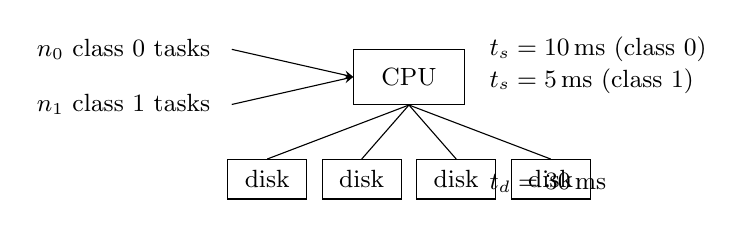
\begin{tikzpicture}[font=\small, line width=0.4pt, >=stealth]
  \node[draw, rectangle, minimum width=1.4cm, minimum height=0.7cm] (cpu) at (0,0) {CPU};
  \node[draw, rectangle, minimum width=1.0cm, minimum height=0.5cm] (d1) at (-1.8,-1.3) {disk};
  \node[draw, rectangle, minimum width=1.0cm, minimum height=0.5cm] (d2) at (-0.6,-1.3) {disk};
  \node[draw, rectangle, minimum width=1.0cm, minimum height=0.5cm] (d3) at (0.6,-1.3) {disk};
  \node[draw, rectangle, minimum width=1.0cm, minimum height=0.5cm] (d4) at (1.8,-1.3) {disk};

  \node[anchor=east] at (-2.4,0.35) {$n_0$ class 0 tasks};
  \node[anchor=east] at (-2.4,-0.35) {$n_1$ class 1 tasks};
  \draw[->] (-2.25,0.35) -- (cpu.west);
  \draw[->] (-2.25,-0.35) -- (cpu.west);

  \draw (cpu.south) -- (d1.north);
  \draw (cpu.south) -- (d2.north);
  \draw (cpu.south) -- (d3.north);
  \draw (cpu.south) -- (d4.north);

  \node[anchor=west] at (0.9,0.35) {$t_s = 10\,\mathrm{ms}$ (class 0)};
  \node[anchor=west] at (0.9,-0.05) {$t_s = 5\,\mathrm{ms}$ (class 1)};
  \node[anchor=west] at (0.9,-1.35) {$t_d = 30\,\mathrm{ms}$};
\end{tikzpicture}
\caption{Central Server Queueing Network}
\end{figure}

To see how the functions described in preceding sections are used, we'll look
at a high-level model of a hypothetical computer system. This system is
represented by the queueing network of Figure 2.1. Networks with this
structure are called central server networks.\footnote{Buzen's development of
efficient computational algorithms for analyzing central server queueing
networks [Buzen 1973] triggered a series of advances in queueing network
analysis methods.}

The system comprises a CPU and four disks. A fixed number of tasks of two
different classes execute in the system, alternating between CPU and disk
activities. There are $n_0$ class 0 tasks, which have a mean CPU execution time
of 10 ms., and $n_1$ class 1 tasks, which have a mean CPU execution time of
5 ms. CPU execution times for both classes are exponentially distributed. CPU
requests of class 1 tasks have preemptive priority over those of class 0 tasks.
If a class 1 task requests the CPU when it is being used by a class 0 task, the
latter is preempted and queued, and the CPU is assigned to the class 1 task.
The interrupted task resumes CPU execution when there are no more class 1
tasks requesting the CPU.

The disk requests of both classes are distributed randomly and uniformly
across all four disks, with the same mean disk service time of 30 ms. Disk
service times are assumed to be Erlang-distributed with a standard deviation
equal to 1/4 of the mean service time.

\paragraph{Open and closed systems.}
The M/M/1 queueing system simulated in Chapter 1 is an open system; customers
arrive from someplace outside the system, are serviced, and leave the system.
The source of customers presumably is unlimited: the probability of a new
customer arriving in the system is not influenced by the number of customers
already in the system, so queues in an open system potentially can grow
without limit. The central server queueing network is a closed system; tasks
receive service at the CPU, at a disk, and then recirculate to request service
at the CPU once again. (The time-sharing system of problem 4, Chapter 1, also
is a closed system.) The maximum queue length at any facility is bounded by
the number of tasks in the system. We can look at this closed network as
representing a fixed-level multiprogramming system with a queue of tasks large
enough so that, whenever a task leaves the system, it is immediately replaced;
the number of tasks executing in the system always remains the same.

Let's assume that the objective of the simulation is to estimate the mean tour
time, or cycle time, for each class. A tour time is the interval between two
successive CPU requests of a task. If we know the mean tour time of a class
and the mean number of tours it makes (mean number of disk requests), we can
compute the mean time a task spends in the system.

\paragraph{The simulation program.}
Figure 2.2 shows a smpl implementation of this model. smpl function names are
underlined in this figure. Preprocessor directives (lines 2--6) define the
number of tasks, the number of disks, and a symbolic representation (gd) for
the value returned by a request or preempt function when a facility
reservation request is queued.

Tokens, in this model, represent tasks. Lines 7--12 define a structure array
of task attributes: these are a task's class, the unit number for the task's
current IO disk request, and the starting time of its current tour. Token
values in smpl function calls in this model are indexes of the element of this
array. Note the array dimensioning: the first element is unused so that we
won't have a token with a 0 value.

The declarations of lines 13--19 define variables used to save descriptors
returned by facility definition functions, to specify the number of tours to be
simulated, and to hold CPU and disk service time distribution parameters.

The first statements of main() initialize variables used to accumulate tour
counts and times for each class. Line 24 sets the class of each task. Lines
25--28 are initialization operations common to all smpl simulation programs:
smpl() is called to initialize the simulation subsystem, facilities are
defined, and the initial events are scheduled. Note that the effect of this
last initialization step is to begin the simulation with all tasks scheduled
for event 1: the simulated system is otherwise empty. This probably is an
unusual system state; we would expect to find tasks distributed throughout the
system (unless there was a major ``bottleneck'' at some point). This state
will be reflected in measurement data collected during the first part of the
simulation run, biasing estimates of steady-state system performance.

\begin{figure}[ht]
\centering
\begingroup\small
\begin{verbatim}
#include <smpl.h>

#define n0 6      /* no. class 0 tasks */
#define n1 3      /* no. class 1 tasks */
#define nt n0+n1  /* total no. of tasks */
#define nd 4      /* no. of disks */
#define gd 1      /* queued req. return */

struct token {
    int cls;   /* task class (& priority) */
    int un;    /* unit for current IO req. */
    real ts;   /* tour start time stamp */
} task[nt+1];

int i, j, event, n[2];
real s[2];
int disk[nd+1], cpu, nts = 10000;
real te[2] = {10.0, 5.0}; /* class 0/1 mean CPU times */
real td = 30.0, sd = 7.5; /* disk time mean, std. dev. */

main()
{
    struct token *p;

    n[0] = n[1] = 0; s[0] = s[1] = 0.0;
    for (i = 1; i <= nt; i++) task[i].cls = (i > n0);

    smpl(0, "central server model");
    cpu = facility("CPU", 1);
    for (i = 1; i <= nd; i++) disk[i] = facility("disk", 1);
    for (i = 1; i <= nt; i++) schedule(1, 0.0, i);

    while (nts) {
        cause(&event, &i);
        p = &task[i];

        switch (event) {
        case 1: /* begin tour */
            p->ts = time();
            schedule(2, 0.0, i);
            break;

        case 2: /* request cpu */
            j = p->cls;
            if (preempt(cpu, i, j) != gd) then
                schedule(3, expntl(te[j]), i);
            break;

        case 3: /* release cpu, select disk */
            release(cpu, i);
            p->un = random(1, nd);
            schedule(4, 0.0, i);
            break;

        case 4: /* request disk */
            if (request(disk[p->un], i, 0) != gd) then
                schedule(5, erlang(td, sd), i);
            break;

        case 5: /* release disk, end tour */
            release(disk[p->un], i);
            j = p->cls;
            s[j] += time() - p->ts;
            p->ts = time();
            n[j]++;
            schedule(1, 0.0, i);
            nts--;
            break;
        }
    }

    printf("class 0 tour time %6.2f\n", s[0] / n[0]);
    printf("class 1 tour time %6.2f\n", s[1] / n[1]);
}
\end{verbatim}
\endgroup
\caption{Queueing Network Simulation Program}
\end{figure}

It is possible to devise more elaborate initialization schemes, but this is
seldom done because of the extra programming effort required. Usually we'll
either discard measurement data collected early in the run or make the run
long enough so that this initialization bias has negligible effects on
results. We'll discuss this problem at some length in Chapter 4.

The length of the simulation run is controlled by nts. When the program is
initialized, this variable is set to the number of tours to be simulated; it is
decremented on each tour completion (line 53) and tested by the while
statement of line 29. Simulation run lengths typically are controlled either
by specifying the simulation time period, as we did in the M/M/1 queue
simulation in Chapter 1, or by specifying an execution count for some
activity. (Also, for certain output analysis methods, runs are terminated when
a specified system state is reached.) Termination on count, rather than time,
is recommended since sample counts are needed in the statistical analysis of
simulation output. We'll usually have a better idea of how many samples we
need than of how much time it will take to collect them.

The cause() function call of line 31 gets the next event together with the
index of the task for which the event is to be executed. This event is then
used to select the appropriate event ``routine'' to execute. Note that a
pointer to the array element for the task is set on line 31.

Event 1 is the start of a tour; the current simulation time is saved as the
tour start time, and event 2 scheduled for immediate occurrence. Event 2
represents a task's CPU request. Remember that a task's class corresponds to
its priority in this model. The preempt() function call requests that the CPU
be reserved for this task. If the CPU currently is reserved by a task of the
same or higher priority, the request is queued, a queued response is returned,
and the event routine simply exited. If the CPU is free, it is reserved for the
requestor. If the CPU is busy with a lower-priority task, that task is
interrupted and queued, and the CPU then reserved for the higher-priority
task. Once the CPU has been reserved for the task, the end of its current CPU
execution interval (event 3) is scheduled. Note that the mean execution
interval is selected according to the task's class.

Two points from our earlier discussion of facility operations bear repeating
here. First, note that recording the tour start time and requesting the CPU
must be done in separate event routines. A blocked CPU request will be queued
and, when the CPU becomes available at some later time, event 2 will be
rescheduled for it. If the tour start time were to be recorded in the same
event routine in which the CPU request is issued, the start time would be
recorded twice: once on the initial CPU request and again on the request's
reexecution. Second, even though events 1 and 2 occur at the same simulation
time, transfer between the two event routines is done indirectly, via a
schedule() call, rather than directly. When cause() returns an event, it
records that event as the current event. If a CPU request is blocked, the
current event number -- event 2 -- is saved in the queue entry created for the
request and, when the CPU becomes available, event 2 is rescheduled. If
control is transferred directly between event routines, smpl loses track of the
current event.

Event 3 marks the completion of a task's CPU execution interval. The CPU is
released, a disk unit selected at random, and the disk request scheduled. If
there are requests queued for the CPU, smpl will dequeue the request at the
head of the queue and return it to execution. There are two possibilities. If
the request was a blocked CPU request, event 2 is scheduled for it at the
current simulation time; reexecution of event 2 will reserve the CPU for the
dequeued request. If the request was a preempted request, the CPU is reserved
for it by smpl, and event 3 is rescheduled for the request.

Event 4 represents the initiation of a task's disk request. (By now it should
be clear why selection of the disk unit and the request for that unit are in
separate event routines.) If the selected unit is busy, the request is queued;
otherwise, the unit is reserved for the requestor and the end of the disk
operation scheduled.

Event 5 is the completion of a task's disk request and of its current tour. The
disk unit is released, the time of the current tour is computed and added to
the accumulated tour times of the task's class, and the count of completed
tours for that class is incremented. The start of the next tour for this task is
scheduled, and the count of the number of tours to be simulated is
decremented. When this count reaches 0, the mean tour times for class 0 and
class 1 are computed and displayed. The values obtained using the random
number generator described in Chapter 8 are 99.34 and 69.37 ms.,
respectively.

Most of the smpl functions described earlier in this chapter are used in this
simulation program, so it is important to understand what the program does
and why it does it. Also, many models will have the same general form as this
one, perhaps with additional facility stages. Similar models are used in other
contexts; for example, the central server network of Figure 2.1 might
represent a memory bus and memory modules, rather than a CPU and disks.
(We'll look at simulation and analytic models of a multiprocessor memory
system in Chapter 5.)

To practice using smpl functions, you may want to try extending this model;
there are a number of possibilities. The level of detail of disk request
processing can be expanded by defining facilities to represent disk
controllers and data channels, decomposing the disk service time into seek,
latency, and transfer times, and adding event routines to initiate and
terminate these activities. The model can be extended to represent
transaction processing by adding an event routine to generate transaction
arrivals and dynamically allocating and deallocating task attribute array
entries as transactions arrive and depart.

\paragraph{A matter of style.}
The format of this and subsequent programs in this book differs in some
respects from common C usage. Differences include the use of then (defined as
empty in smpl.h) and the positioning of braces. This reflects only the
author's preference in program style and not any advocacy of style. In moving
the smpl source code in the Appendix to your system, you should feel free to
reformat it according to your own preference.

\section{Debugging Aids}
\label{sec:smpl-debugging-aids}

\paragraph{Error messages.}
Various errors are detected by smpl. When an error is detected, smpl displays
or prints an error message, generates a simulation report (if the current
output destination is the printer), and terminates simulation program
execution. Error messages give the simulation time at which the error was
detected and one of the following diagnostic clauses.

\begin{verbatim}
empty element pool
empty name space
facility defined after queue/schedule
negative event time
empty event list
preempted token not in event list
release of idle/unowned facility
stream argument error
uniform argument error: a > b
random argument error: i > j
erlang argument error: s > x
hyperx argument error: s not > x
\end{verbatim}

smpl maintains a common pool of elements from which the event list and data
structures for facilities and queues are constructed. The size of this pool is
fixed when smpl is compiled. An empty element pool error occurs when the
total number of static and dynamic entities for which pool elements must be
allocated exceeds the size of the pool. Sometimes this simply is due to the
size of the model, and the only cure is to increase the size of the pool. It
frequently is caused by a ``runaway'' simulation program which generates
arrivals but not departures. A second pool is used to hold model and facility
names; when this pool is filled, an empty name space error occurs. You can
shorten the names or increase the size of this pool.

An error occurs if a facility is defined after an event has been scheduled or a
facility request queued (for reasons which have to do with data structure
creation). Sequencing model operations in the required order will eliminate
this error.

Scheduling an event with a negative inter-event time usually results from some
kind of computation problem (but remember that variates from the normal
distribution can be negative).

An error occurs when cause() finds the event list empty, usually because a
scheduling operation was forgotten someplace (and sometimes because we've
unwittingly modeled a deadlock situation).

When a token's use of a facility is preempted by a higher-priority token, smpl
searches the event list to find an entry for the token being preempted. It
assumes that this entry represents the end of the token's execution interval
on that facility, and suspends the remaining part of the interval until the
facility is once again available for that token. An error occurs if the
preempted token can't be found in the event list. This usually results from a
program bug, but sometimes results from model complexities which exceed the
restrictions imposed by smpl's implicit queueing.

When a facility is released, smpl verifies that the token specified in a
release() call is the same as the reserving token: if it is not, an error
occurs. This catches a surprising number of program bugs.

The remaining errors in this list result from invalid arguments in random
number generator function calls and were described earlier.

The above errors result in calls to the smpl function

\begin{verbatim}
error (n, s);
int n; char *s;
\end{verbatim}

which also can be called from a simulation program. You may want to do this to
generate a simulation report on a program-detected error. In this case, n (an
error code used by smpl) should be 0, and s should point to a string
containing the diagnostic clause you want included in the error message. An
error message always is displayed on the screen; if the current output
destination is the printer, it also is printed, followed by the simulation
report. (Output destination control is described later on in this chapter.)

\paragraph{Traces.}
When the cause of an error isn't obvious from an examination of the program,
we can use the smpl trace to get additional information. Tracing is controlled
by calls to the following function.

\begin{verbatim}
trace (n);
int n;
\end{verbatim}

n, the trace control flag, should be in the range 0--4; any other value is
ignored. Values in the range 1--3 turn tracing on; a 0 value turns tracing off.

\begin{figure}[ht]
\centering
\begingroup\small
\begin{verbatim}
time 79.898 -- token 7 -- CAUSE EVENT 5
- token 7 -- RELEASE disk
- token 7 -- SCHEDULE EVENT 1
- token 7 -- CAUSE EVENT 1
- token 7 -- SCHEDULE EVENT 2
- token 7 -- CAUSE EVENT 2
- token 7 -- PREEMPT CPU: INTERRUPT
-- SUSPEND EVENT 3
-- QUEUE token 4 (inq = 3)
-- RESERVE CPU for token 7
- token 7 -- SCHEDULE EVENT 3

time 87.828 -- token 7 -- CAUSE EVENT 3
- token 7 -- RELEASE CPU
-- DEQUEUE token 4 (inq = 2)
-- RESERVE CPU for token 4
-- RESUME EVENT 3
- token 7 -- SCHEDULE EVENT 4
- token 7 -- CAUSE EVENT 4
- token 7 -- REQUEST disk QUEUED (inq = 1)

time 96.976 -- token 2 -- CAUSE EVENT 5
- token 2 -- RELEASE disk
-- DEQUEUE token 7 (inq = 0)
-- RESCHEDULE EVENT 4
- token 2 -- SCHEDULE EVENT 1
- token 7 -- CAUSE EVENT 4
\end{verbatim}
\endgroup
\caption{smpl Trace Message Sequence}
\end{figure}

If n is 1, the trace is free-running; trace messages are generated
continuously on the screen or printer, depending on the current output
destination. If n is 2, trace messages are sent to the screen; execution is
paused whenever the screen fills. If n is 3, trace messages also are sent to
the screen but with a pause after every message. In both cases, execution is
resumed following a pause by pressing any key. User trace messages can be
intermingled with smpl trace messages. After each user trace message is
displayed or printed, a trace(4) call will cause smpl to update line counts and
issue a page change or screen pause if appropriate.

When the error occurs early in the execution of our simulation program, we can
turn tracing on as part of model initialization and step through model
execution, screen by screen, until the error occurs. After we get the early
(and usually easy) bugs out, and encounter errors later in the simulation,
this approach becomes too time-consuming. We can add an event routine to our
simulation program which, when the corresponding event occurs, will turn
tracing on. During initialization, we schedule that event to occur some time
earlier than the error; how much earlier is a matter of guesswork -- the error
and its cause may be far apart in time.

When tracing is on, messages are generated whenever a facility is defined,
requested, or released, and whenever an event is scheduled or caused. Trace
messages give the time at which the operation occurred (if it has changed
since the previous trace message) and identify tokens involved in the
operation. Messages for schedule and cause operations give the associated
event number. Messages for facility request and release operations give the
facility name and the current queue length at the facility, and show the
queueing and dequeueing of tokens.

Figure 2.3 shows a sequence of trace messages from the execution of the
simulation program of Figure 2.2. This sequence traces the execution of a
token from the completion of one disk request up to its initiation of its next
disk request. This token -- token 7 -- represents a higher-priority (class 1)
task.

The trace sequence begins at the end of a tour for token 7: event 5 occurs, the
disk is released, and event 1 scheduled. There is no inter-event delay between
event 5 and event 1, so event 1 occurs immediately (event 1 simply records the
tour start time), and event 2 is scheduled. Again, there is no delay between
events 1 and 2, so event 2 occurs immediately. Event 2 is a CPU request. Since
the CPU is reserved by a lower-priority token, token 4, preemption takes
place. The event 3 scheduled for token 4 is suspended, token 4 is placed on
the CPU queue (whose length now becomes 3), and the CPU is reserved for token
7. Token 7 then schedules its release of the CPU, event 3. Note that all these
operations take place at the same point in simulation time.

In this particular sequence, there are no intervening events between events 2
and 3 of token 7. When its event 3 occurs, token 7 releases the CPU. Token 4,
which was interrupted earlier, is dequeued (reducing the CPU queue length to
2), the CPU is reserved for it, and its suspended execution interval resumed.
Token 7 schedules event 4 and, on its occurrence, issues its disk request. This
request finds the disk unit busy and is queued; note that it is the only
request queued for this unit.

The next event to occur is the completion of a disk request for token 2. When
this token releases the disk, token 7 is dequeued and event 4 rescheduled for
it. After token 2 has scheduled the start of its next tour, token 7's disk
request (event 4) is reinitiated.

smpl trace messages usually provide enough information to pinpoint problems in
simple simulation programs. However, while these messages can show which
operations are performed, they can't show why; as program complexity
increases, so does the need for user-level debugging aids. If you get involved
in developing large simulation models, build in debugging facilities from the
start.

SMPL debugging aids. SMPL provides several facilities to help speed debugging.
Simulation time is continuously displayed on the screen, and execution can be
paused at any time by pressing a key. For more precise control, a breakpoint
can be set from the keyboard to pause execution at a specified time or a
specified parameter value is reached. Tracing can be turned on and off via
function keys. SMPL provides a ``dump'' capability, which displays the state
of the simulated system, including facility status and users, queue entries,
and event list contents (an example appears in Section 7.4). The dump display
can be generated at any time from the keyboard; it also is generated whenever
an error occurs. The ability to control basic debugging aids from the keyboard
greatly reduces the amount of time spent modifying and recompiling simulation
programs.

\section{Data Collection and Reporting}
\label{sec:smpl-data-collection-reporting}

smpl collects data on facility utilization and queueing, and uses this data to
produce the simulation report. This report gives the utilization, mean busy
period, mean queue length, and release, preempt, and queue operation counts
for each facility. The reported measures represent operations completed from
the start of the current measurement interval up to the time of the report. The
measurement interval starts at simulation time 0 unless the reset() function
is called. reset() clears facility counters and accumulators, discarding
measurement data collected up to the time of its call, and sets the start of
the measurement interval to the current simulation time. The simulation report
is generated and sent to the current output destination by the following
function call.

\begin{verbatim}
report ();
\end{verbatim}

This function generates the simulation report and sends it to the current
output destination. Figure 2.4 shows the simulation report obtained by adding
a report() function call to the simulation program of Figure 2.2. The report
heading includes the model name, the current simulation time, and the
measurement interval length (which corresponds to the simulation period in
this case). Facility names are those specified in facility() function calls. In
this model, all facilities have single servers. For a multi-server facility,
the number of servers is appended in brackets to the facility name.

\begin{figure}[ht]
\centering
\begingroup\small
\begin{verbatim}
smpl SIMULATION REPORT

MODEL: central server model      TIME 29652.553

INTERVAL: 29652.553

MEAN BUSY   MEAN QUEUE   OPERATION COUNT
FACILITY     UTIL  PERIOD LENGTH   RELEASE PREEMPT QUEUE
CPU          0.8151 6.202 1.2286    12687   2682   7335
disk         0.7872 29.970 0.933    2484    0      1838
disk         0.7161 29.704 0.847    2457    0      1787
disk         0.7804 29.844 0.921    2514    0      1896
disk         0.7886 30.029 0.951    2939    0      1931
\end{verbatim}
\endgroup
\caption{smpl Simulation Report}
\end{figure}

The utilization of a facility is computed by dividing the accumulated busy
time of all servers by the length of the measurement interval; the
utilization of a multi-server facility may be greater than 1. Busy times are
accumulated when a server is released, so the utilization does not reflect
facility execution intervals in progress at the time of the report. This end
effect usually is insignificant because of the relative length of the run, but
should be kept in mind when using a report covering a small simulation period
in debugging.

The mean busy period is computed by dividing the accumulated busy time by the
release count. The release count is the sum of release operations effected via
a release() call and those resulting from facility preemption. For
non-preemptable facilities, the reported mean busy period should be
approximately equal to the mean facility execution interval specified in the
simulation program. Note that the mean disk busy periods in this report are
very close to the specified mean disk service time of 30 ms.

For preemptable facilities, the reported mean busy period is not necessarily
 the same as the mean execution interval, since it reflects interrupted
intervals. However, we can compute the mean execution interval from the
reported data. The product of the mean busy period and the release count (or
 the product of the utilization and the measurement interval) gives the total
busy time. The preempt count is the number of actual preemptions which
occurred, so the difference between the release count and the preempt count
is the number of completed execution intervals. Dividing the total busy time by
this number gives the measured mean execution interval.

Let's compare the measured mean CPU execution interval with that we'd expect
from the values specified in the simulation program. From the report data, the
mean interval is (6.202 x 12687) / (12687 - 2682) = 7.865 ms. The two classes
of tasks in this model have different mean CPU execution times; to compute an
overall mean, we need counts of the number of completed CPU execution
intervals for each class. We can obtain values very close to these counts by
adding statements to the simulation program to print the class 0 and class 1
tour counts, n[0] and n[1]. For this particular implementation, these are 5827
and 4173. The mean CPU times specified for class 0 and class 1 are,
respectively, 10 ms. and 5 ms., so we'd expect an overall mean of
(5827 x 10 + 4173 x 5) / 10000 = 7.914 ms. The measured mean of 7.865 ms. is
very close to this value.

The mean queue length of a facility is the average number of tokens in the
facility's queue; it does not include tokens in service. The mean queue length
is computed using the method described in Section 1.5. The mean number of
tokens in queue and in service at a facility is the sum of the facility
utilization and the mean queue length. The sum of utilizations and mean queue
lengths for all facilities is the mean number of tokens in the system (for the
report of Figure 2.4, the sum is 8.9994).

The release count is the sum of all facility releases, including those
resulting from preemption. The preempt count is the number of actual
preemptions (not the number of preempt() function calls). The number of
complete facility operations is the difference between the release count and
the preempt count. This number, divided by the measurement interval length,
is the facility's throughput. The average time in queue at a facility can be
computed by dividing the mean queue length by the throughput of the facility.

The queue count is the number of dequeue operations performed during the
measurement interval. It includes requests queued because the facility was
busy and requests queued after preemption. The difference between the queue
count and the preempt count is the number of blocked requests.

Sometimes you'll want to develop a report tailored to a particular model. The
U(), B(), and Lq() functions described in Section 2.4 (together with the
operational relationships discussed in Section 1.4) can help in doing this.

\paragraph{SMPL Reports.}
SMPL provides additional data collection and reporting tools. These include
the table facility, used to collect, tabulate, and plot distributions of model
variables, and the time series display, used to plot a variable such as average
or instantaneous queue length versus time. With SMPL, any report can be
displayed at any time simply by pressing a function key. We'll look at the
design of the table facility in Chapter 9.

\section{Output Control}
\label{sec:smpl-output-control}

Error and trace messages, and the simulation report, are sent by smpl to the
current output destination. This destination is initially set to stdout.
(Turning tracing on with a trace control flag of 2 or 3 also sets the output
destination to stdout.) You can redirect output to the printer or a disk file,
or find out what the current destination is, via a call to the following
function.

\begin{verbatim}
p = FILE *sendto (dest);
FILE *dest;
\end{verbatim}

If dest is null, sendto() returns the file pointer of the current destination.
If it is not null, the associated file becomes the current output destination.

\section{Summary}
\label{sec:smpl-summary}

This chapter has described the simulation, debugging, and reporting functions
of smpl, and discussed their use in a queueing network simulation program.
We'll look at more smpl simulation programs in Chapters 5 and 6. If you have
questions about any of these functions, read the appropriate section on
implementation in Chapter 8, or check the source code in the Appendix. The
simulation functions discussed in this chapter are summarized in Figure 2.5. A
few utility functions were not described here; you'll come across these in
moving smpl to your system. (When this move is accomplished, you can use the
program of Figure 2.2 as a test case. If you use the same random number
generator, you should be able to reproduce exactly the mean tour values, the
trace sequence, and the simulation report.)

If the subject of operational analysis (introduced in Section 1.4) is new to
you, it would be a very useful exercise to read Chapters 2 and 3 of Lazowska
et al.\ [1984] and apply the relationships discussed in these chapters to the
analysis of the output from this model. Go through the arithmetic to compute
throughputs, queueing times, and residence times at each facility, and for
 each class at the CPU. This may seem just a matter of bookkeeping (and in
some respects it is), but an understanding of these relationships is very
important in model development and testing, and sometimes will eliminate the
need to build a model at all.

\begin{figure}[ht]
\centering
\begingroup\small
\begin{verbatim}
INITIALIZATION

smpl (0, s)      initialize simulation subsystem
reset ()         clear measurement counters & accumulators

FACILITY DEFINITION, OPERATION, AND QUERY

f = facility (s, n)  define facility & return descriptor
r = request (f, j, p) reserve facility: r = 1 if queued
r = preempt (f, j, p) preempt facility: r = 1 if queued

release (f, j)   release facility & dequeue request
r = status (f)   get current facility status: r = 1 if busy
n = inq (f)       get current queue length
u = U (f)         get utilization
b = B (f)         get mean busy period
l = Lq (f)        get queue mean length

EVENT SCHEDULING

schedule (e, t, j) schedule event
cause (e, j)       cause event (e, j are pointers)
j = cancel (e)     cancel event & return token
t = time ()        get current simulation time

DEBUGGING AND REPORTING

trace (n)          set trace mode
error (n, s)       display error message & halt
report ()          generate simulation report

lcnt (n)           count output lines on current page
endpage ()         advance (pause) on full page (screen)
newpage ()         initialize page/screen line count
d = sendto (d)     get/set output destination

RANDOM VARIATE GENERATION

n = stream (n)     set/get random number stream number
v = ranf ()        generate uniform [0,1] variate
v = uniform (a, b) generate uniform [a,b] variate
v = expntl (x)     generate exponential variate
v = erlang (x, s)  generate Erlang variate
v = hyperx (x, s)  generate hyperexponential variate
v = normal (x, s)  generate normal variate
k = random (i, j)  generate random integer
\end{verbatim}
\endgroup
\caption{smpl Function Summary}
\end{figure}

\section{Problems}
\label{sec:smpl-problems}

\begin{enumerate}
\item Run the M/M/1 queue simulation model of Figure 1.7 and use the data
provided by the smpl simulation report to compute the system throughput $X$
and mean residence time $W$. Replace the server in this model by two servers
operating at one-half the speed of the original single server (doubling $T_s$),
run the revised model, compute $X$ and $W$ for this M/M/2 queue, and compute
the ratio of residence times for the two systems. (Both systems have the same
expected throughput $1/T_a$.) Increase the system load by reducing $T_a$ to
125.0, and repeat the two runs; what happens to the residence time ratio?

\item Extend the M/M/1 queue model of Figure 1.7 to provide a preemptive
priority queueing discipline. Assume there are two independent customer
classes: both have mean inter-arrival times of 400 units and mean service times
of 100 units, but class 2 customers have higher priority than class 1
customers. Implement some type of customer descriptor record so that arriving
customers can be marked with their class and arrival time; instrument the
model to compute and report the mean residence time for each class and for all
customers. Run this model using the same simulation period as the model of
Figure 1.7, and compare the values of $W$ obtained for the combined classes
with that obtained for the M/M/1 queue with first-come, first-served queueing.

\item A simple timesharing system model. A timesharing system (problem 4,
Chapter 1) has 16 user terminals connected to a computer system with two
identical disks. Figure 2.6 shows a queueing diagram of this system. Workload
characteristics are the same for all 16 users; user think times have a
negative exponential distribution with a mean think time $Z$ of 5 seconds.

Processing of a terminal request requires a mean CPU time of 480 milliseconds
(ms.) and an average of 12 disk requests. The mean CPU execution interval per
disk request therefore is 40 ms. Inter-disk-request intervals are
exponentially distributed. For modeling purposes, it can be assumed that, when
a disk request completes, another CPU execution interval is initiated with
probability $p_x$ or terminal request processing is completed (and another
think time initiated) with probability $1 - p_x$. $p_x$ is defined as
$1 - 1/n_{io}$, where $n_{io}$ is the average number of disk requests per
terminal request. ($n_{io} = 12$, then, in this case.)

Disk requests are distributed randomly, independently, and uniformly across
the two disks. The service time for a disk request is the sum of seek, latency,
and transfer times; data is transferred in units of one block (or sector).
Disks have a revolution time of 16.7 ms., a minimum seek time of 0 ms., a
maximum seek time of 50 ms., and a transfer time of 0.52 ms. per block. While
 the mean seek time is not known, observation indicates that most seek times
are in the vicinity of 16 ms., so it is assumed that the seek time distribution
can be modeled by a triangular distribution with range [0, 50] ms. and mode
16 ms. (see problem 3, Chapter 1). Latency times are distributed uniformly in
[0, 16.7] ms., and disk requests transfer one block of data.

\begin{figure}[ht]
\centering
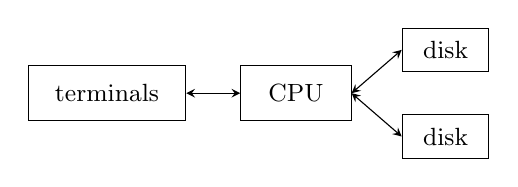
\begin{tikzpicture}[font=\small, line width=0.4pt, >=stealth]
  \node[draw, rectangle, minimum width=2.0cm, minimum height=0.7cm] (terms) at (-2.4,0) {terminals};
  \node[draw, rectangle, minimum width=1.4cm, minimum height=0.7cm] (cpu) at (0,0) {CPU};
  \node[draw, rectangle, minimum width=1.1cm, minimum height=0.55cm] (d1) at (1.9,0.55) {disk};
  \node[draw, rectangle, minimum width=1.1cm, minimum height=0.55cm] (d2) at (1.9,-0.55) {disk};

  \draw[<->] (terms.east) -- (cpu.west);
  \draw[<->] (cpu.east) -- (d1.west);
  \draw[<->] (cpu.east) -- (d2.west);
\end{tikzpicture}
\caption{Timesharing System Queueing Diagram}
\end{figure}

Build a smpl model of this system, instrumenting the model to collect terminal
request response times and to report the mean response time. All queues have
first-in, first-out queueing. Make a simulation run of 2000 terminal requests
and perform an operational check of the results, using utilizations and queue
lengths from the smpl simulation report to verify the mean response time.
Determine the mean number of terminal requests in the system.

\item Representing memory. The above model has no provision for representing
the effect of memory capacity on response time. The simplest way to represent
memory is to assume that the system has a multiprogramming level (mpl) of $m$
active users. When a terminal sends a request to the system, that request is
accepted by the system and its execution initiated if the number of requests
currently being executed is less than $m$; otherwise, the system queues the
request until one of the $m$ executing requests complete. Assume the system
has a mpl of 6, and add memory queueing to your model. (One possibility is to
represent memory as a facility with 6 servers.) Make a simulation run of 2000
terminal requests and perform an operational analysis of the results. Compute
the response time components: memory waiting time, mean CPU residence time per
terminal request, and mean disk residence time per terminal request. Compare
the mean response time and mean number of requests in the system with those
obtained for the model of problem 3.

\item Representing swapping. The work performed by a user at a terminal in
this system involves a continuing series of interactions between the user and a
program executing in the computer system. Each user interacts with a different
program (or, equivalently, with a different instance of a common program). To
execute, a program requires memory and certain logical resources which,
collectively, are called an address space. It is assumed that the
multiprogramming level, or mpl, specifies the number of address spaces in the
computer system.

The program assigned to a given address space is said to be resident.
Resident programs have two states: active and dormant. A program is active
while executing and dormant when it has completed execution and returned a
response to the terminal. When the system receives a terminal request, it
determines if the user's program is resident. If it is, the program is
scheduled for execution. If it is not, and there is an address space
containing a dormant program, the system swaps out the dormant program to disk
and swaps in the requested program to that address space.

Extend the model of problem 4 to represent swapping, based on the following
assumptions. The computer system has 6 address spaces. (These can be
represented by a facility with 6 servers; a server is reserved when the
program in an address space becomes active and released when the program
becomes dormant.) When a terminal request arrives for a non-resident program
and all address spaces contain active programs, the request is queued until one
of these programs becomes dormant and an address space can be assigned to the
request. The system then swaps out the dormant program and swaps in the
program being activated. If a request for a non-resident program finds several
address spaces with dormant programs, it swaps out the program which has been
dormant the longest.

The number of disk blocks transferred by a swapout is assumed to be
distributed uniformly between 30 and 60. The system chooses a swapout
destination disk at random; if the chosen disk is busy, the swapout is
assigned to the other disk regardless of that disk's status. The number of
blocks and source disk for a program's swapin are established when the
program is swapped out. The operating system serializes swap operations so
that only one swap, in or out, is in progress at any one time by placing
swapout and swapin requests on a FIFO queue. (A smpl facility can be used to
represent this queue.) If a terminal request arrives to find its program being
swapped out to accommodate an earlier arrival, the swapout is allowed to
complete. If an address space is available, it is assigned to the
newly-arrived request and a swapout initiated for the dormant program in that
address space. Since swaps are serialized, the swapin of the program for this
request will not be initiated until its swapout completes.

Make a simulation run of 2000 terminal requests. Compute the response time
components as before (keep in mind that swap queue delays and disk transfers
for swapouts do not contribute to the response time except when a program
swapin has to wait on its own swapout).

\item Incorporating CPU scheduling. Suppose terminal requests are classified,
more or less arbitrarily, as class 0 or class 1, depending on whether their CPU
time requirements are less than or greater than 250 ms. Instrument the model
of problem 5 to report response times by class, as well as the overall response
time.

\begin{enumerate}
\item Some systems use round-robin (RR) CPU scheduling so that a request for a
small amount of CPU time will not be disproportionally delayed by execution of
a request requiring a large amount of CPU time. With RR scheduling, the CPU is
cyclically allocated to the requests in the CPU queue. Each request, in turn,
receives CPU service for a fixed quantum of time (or for the time remaining in
its current execution interval, if smaller than a quantum). Incorporate RR
scheduling in the model of problem 5, using a quantum time of 25 ms. Simulate
2000 terminal requests. Compare the results with those obtained in problem 5.
What effect did the incorporation of RR scheduling have? Why?

Note that if your version of smpl uses 16-bit ints, the large number of CPU
operations required in simulating this system with RR scheduling will cause
some counters associated with the CPU facility to overflow, so that some
reported CPU measures will be meaningless. To circumvent this, generate a
simulation report and reset smpl after every 32767 CPU releases, and merge the
reports by hand at the end of the run. Alternatively, use the U(), B(), and
Lq() functions to get facility measures after every 32767 CPU releases, and
write a function to merge and report these measures.

\item Suppose the system attempts to favor class 0 requests by computing CPU
request priority based on accumulated CPU time as follows:

\begin{verbatim}
priority = max(0, 10 - [0.01 * accumulated CPU time])
\end{verbatim}

where [x] denotes the floor function of x -- the largest integer equal to or
less than x. Thus, a request is assigned a priority of 10 upon arrival, and its
priority is reduced by 1 whenever it accumulates another 100 ms. of CPU time
until it has been reduced to 0. Incorporate this scheduling algorithm into the
model of problem 5 (no RR scheduling) and simulate 2000 terminal requests.
Compare the mean response time of class 0 requests with that obtained without
priority scheduling. What can be done to improve the response time of class 0
requests? How would you model the proposed improvement?
\end{enumerate}
\end{enumerate}
